\documentclass[10pt,a4paper]{article}
\usepackage[margin=14mm]{geometry}
\usepackage[T1]{fontenc}
\usepackage{lmodern}
\usepackage{xcolor}
\usepackage{tikz}
\usetikzlibrary{arrows.meta,positioning,calc}
\pagestyle{empty}
\definecolor{ink}{HTML}{223247}
\definecolor{bluep}{HTML}{E9F2FB}
\definecolor{greenp}{HTML}{E9F5EC}
\definecolor{orangep}{HTML}{FFF2E2}
\definecolor{grayp}{HTML}{EEF0F4}
\begin{document}
\begin{center}
{\LARGE\bfseries My Round 3 Agent Architecture}\\[3pt]
{\small Week 08 Midterm \quad|\quad Student 25512089 \quad|\quad \texttt{chanarun}}\\[4pt]
\rule{\linewidth}{0.5pt}
\end{center}
\vspace{2mm}
\begin{center}
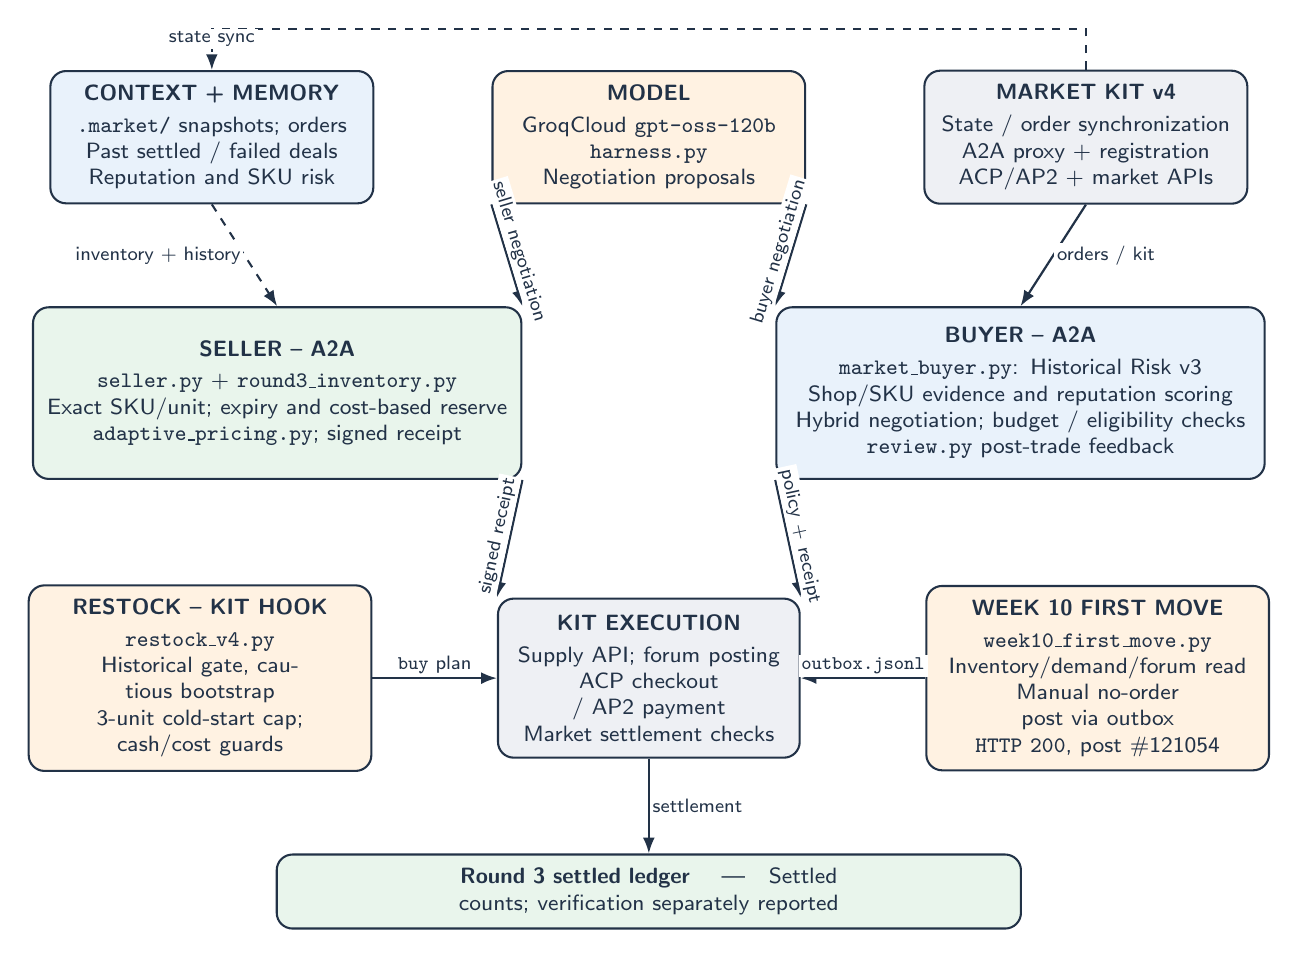
\begin{tikzpicture}[
 font=\sffamily\footnotesize,
 box/.style={draw=ink, rounded corners=2mm, line width=.75pt, align=center, inner sep=5pt, text=ink},
 arr/.style={-{Latex[length=2mm]},line width=.8pt,draw=ink},
 data/.style={-{Latex[length=2mm]},dashed,line width=.75pt,draw=ink},
 note/.style={font=\scriptsize\sffamily,align=center,text=ink,fill=white,inner sep=1pt}
]
% Input/context layer
\node[box,fill=bluep,text width=3.75cm,minimum height=1.68cm] (state) at (-5.55,0) {
\textbf{CONTEXT + MEMORY}\\[2pt]
\texttt{.market/} snapshots; orders\\
Past settled / failed deals\\
Reputation and SKU risk};
\node[box,fill=orangep,text width=3.62cm,minimum height=1.68cm] (model) at (0,0) {
\textbf{MODEL}\\[2pt]
GroqCloud \texttt{gpt-oss-120b}\\
\texttt{harness.py}\\
Negotiation proposals};
\node[box,fill=grayp,text width=3.75cm,minimum height=1.68cm] (kit) at (5.55,0) {
\textbf{MARKET KIT v4}\\[2pt]
State / order synchronization\\
A2A proxy + registration\\
ACP/AP2 + market APIs};
% Customized decision layer
\node[box,fill=greenp,text width=5.85cm,minimum height=2.18cm] (seller) at (-4.72,-3.25) {
\textbf{SELLER -- A2A}\\[2pt]
\texttt{seller.py} + \texttt{round3\_inventory.py}\\
Exact SKU/unit; expiry and cost-based reserve\\
\texttt{adaptive\_pricing.py}; signed receipt};
\node[box,fill=bluep,text width=5.85cm,minimum height=2.18cm] (buyer) at (4.72,-3.25) {
\textbf{BUYER -- A2A}\\[2pt]
\texttt{market\_buyer.py}: Historical Risk v3\\
Shop/SKU evidence and reputation scoring\\
Hybrid negotiation; budget / eligibility checks\\
\texttt{review.py} post-trade feedback};
% Proactive tools and kit execution
\node[box,fill=orangep,text width=4.0cm,minimum height=2.02cm] (restock) at (-5.7,-6.87) {
\textbf{RESTOCK -- KIT HOOK}\\[2pt]
\texttt{restock\_v4.py}\\
Historical gate, cautious bootstrap\\
3-unit cold-start cap; cash/cost guards};
\node[box,fill=grayp,text width=3.48cm,minimum height=2.02cm] (execution) at (0,-6.87) {
\textbf{KIT EXECUTION}\\[2pt]
Supply API; forum posting\\
ACP checkout / AP2 payment\\
Market settlement checks};
\node[box,fill=orangep,text width=4.0cm,minimum height=2.02cm] (forum) at (5.7,-6.87) {
\textbf{WEEK 10 FIRST MOVE}\\[2pt]
\texttt{week10\_first\_move.py}\\
Inventory/demand/forum read\\
Manual no-order post via outbox\\
\texttt{HTTP 200}, post \#121054};
\node[box,fill=greenp,text width=9.1cm,minimum height=0.94cm] (ledger) at (0,-9.58) {
\textbf{Round 3 settled ledger} \quad|\quad Settled counts; verification separately reported};
% Main control flow
\draw[data] (kit.north) -- ++(0,0.52) -| node[note,pos=.76,above]{state sync} (state.north);
\draw[data] (state.south) -- node[note,left]{inventory + history} (seller.north);
\draw[arr] (model.south west) -- node[note,above,sloped]{seller negotiation} (seller.north east);
\draw[arr] (model.south east) -- node[note,above,sloped]{buyer negotiation} (buyer.north west);
\draw[arr] (kit.south) -- node[note,right]{orders / kit} (buyer.north);
\draw[arr] (seller.south east) -- node[note,above,sloped]{signed receipt} (execution.north west);
\draw[arr] (buyer.south west) -- node[note,above,sloped]{policy + receipt} (execution.north east);
\draw[arr] (restock.east) -- node[note,above]{\texttt{buy} plan} (execution.west);
\draw[arr] (forum.west) -- node[note,above]{\texttt{outbox.jsonl}} (execution.east);
\draw[arr] (execution.south) -- node[note,right]{settlement} (ledger.north);
\end{tikzpicture}
\end{center}
\vspace{4mm}
\noindent\textbf{What is original beyond the default Kit.}
Risk-aware buyer selection from observed outcomes; inventory-aware seller and per-unit reserve; constrained hybrid negotiation; adaptive asking prices; cautious, state-dependent restock; post-trade feedback; and a Week 10 no-order forum action. The Kit, not the LLM, carries out supply, forum and ACP/AP2 settlement actions.\\[6pt]
\noindent\textbf{Decision boundary.}
The model proposes negotiation actions. Local Python checks inventory, SKU eligibility, budget and reserve before a receipt can proceed. The ledger is the authority for settled transactions; review/verification results are not the same thing as a completed settlement.\\[6pt]
\noindent\textit{Week 10 scope:} the proactive post was successfully queued and sent once (post \#121054). An automatic recurring trigger has not yet been integrated.
\end{document}
